\documentclass[conference]{IEEEtran}

\usepackage{cite}
\usepackage{amsmath}
\usepackage{url}
\usepackage{pdfpages}
\usepackage{soul}

% for comments
\usepackage{color}
\newcommand{\mycomment}[3]{\emph{\textcolor{#2}{#1}: }\textcolor{#2}{#3}}
\newcommand{\todo}[1]{\mycomment{Todo}{red}{#1}}
\newcommand{\sangeetha}[1]{\mycomment{Sangeetha}{magenta}{#1}}
\newcommand{\eric}[1]{\mycomment{Eric}{cyan}{#1}}

% correct bad hyphenation here
\hyphenation{op-tical net-works semi-conduc-tor}


\begin{document}
% paper title
\title{Perceptron-Based Prefetch Filtering in Gem5\\ CS752 Project Progress Report}


% author names and affiliations
% use a multiple column layout for up to three different
% affiliations
\author{
\IEEEauthorblockN{Sangeetha Grama Srinivisan}
\IEEEauthorblockA{University of Wisconsin, Madison\\
Email: \texttt{sgsrinivasa2@wisc.edu}}
\and
\IEEEauthorblockN{Eric Brandt}
\IEEEauthorblockA{University of Wisconsin, Madison\\
Email: \texttt{elbrandt@wisc.edu}}}

% make the title area
\maketitle

\section{Introduction}
Prefetching has been used as an effective strategy to improve processor performance. Many prefetching strategies are proposed based on spatial or temporal access patterns observed in the program. Machine learning algorithms ranging from simple perceptrons to complex LSTM (Long-Short-Term-Memory) models are leveraged to design and optimise prefetching strategies. One such design uses a perceptron-based prefetch filter\cite{ppf} to enhance Signature Path Prefetching \cite{SPP}, a lookahead prefetcher. In this project we aim to implement this perceptron-based prefetch filter\cite{ppf} in GEM5 \cite{lowepower2020gem5} simulator and evaluate the performance implications of the filtered prefetches on a wide range of workloads. 

\section{Relevance}
Memory accesses span over multiple cycles. The rate of improvement in memory access speeds compared to the rate of improvement in processor speeds indicates that there is a wide gap known as the Memory Wall \cite{mem-wall}. This significant difference in speeds can be mitigated by prefetching memory into the cache. The prefetching strategies are continuously optimised to improve accuracy of prefetching while also maintaining a good coverage, i.e, the prefetcher should be able to eliminate cache misses and all the prefetched memory should be used by the processor. While the former requirement focuses on improving processor performance, the latter requirement helps conserve memory bandwidth and the space availability in the cache. Machine learning algorithms have been used to improve or enhance prefetching, like, offline parameter optimisation for baseline prefetchers or on-line parameter tuning to provide feedback to the prefetcher based on the result of the prefetch, such as the perceptron-based prefetch filter\cite{ppf}. Implementing this filter in GEM5 will help in getting a detailed analysis of performance implications on a wide range of program workloads and architectures.  Further, the prefetch filter can be used as a standalone unit with any baseline prefetcher, giving researchers the opportunity to explore the use of this filter with their designs.

\section{Planned Evaluation Methods}

Implementation success will be measured both qualitatively and quantitatively. The \textit{qualitative} evaluation will verify that the Perceptron Prefetcher algorithm is implemented \textit{correctly} (e.g, behaves in a manner consistent with the proposed design, and does not contain bugs). This will be achieved through a combination of custom log (stat) files generated during runtime that are inspected post-mortem, and carefully crafted sample workloads designed to elicit certain behaviors of the prefetcher to exercise all possible code paths. 

The \textit{quantitative} evaluation will involve a set benchmarks that include broad scope workloads (e.g. SpecXX), and some numerically intensive benchmarks specific to the domain of physics based animation. As a departure from our proposal, we have decided that comparing results to other prefetch research will not be easy or feasible. It will be difficult to replicate exact simulation conditions of other research, especially considering a simulator other than Gem5 was used in many of the prefetcher related research papers. Instead, we will quantitatively compare the performance of our perceptron prefetcher implementation with the existing Gem5 prefetcher, and examine its effect on different CPUs, different benchmarks, and possibly different cache sizes and configurations.  

\section{Related Work}

We can broadly classify prefetching mechanisms into 2 categories - Spatial prefetching and Look-ahead prefetching. The former does not take into account the order of accesses while the latter does. One such spatial prefetcher is the AMPM\cite{AMPM}, which proposes Access Map Pattern Matching to generate and issue prefetches. As the name suggests, the mechanism uses pattern matching to identify memory access pattern and generate prefetch requests. In order to do so, the main memory is partitioned into many zones, and 'hot-zones' are identified based on the latest memory accesses issued from the CPU. A map is used to store the memory accesses in these zones, with the help of which a pattern, which is nothing but the stride, is determined. For each line in the zone, the map uses a 2 bit value to track the accesses: Init/Prefetch/Access/Success. These states along with the identified access pattern of that zone are used to issue prefetches.  

Pugsley et al. present a prefetching technique known as Sandbox Prefetching\cite{sandbox}, which is another spatial prefetcher. The design first uses global pattern confirmation of the cache accesses using a bloom filter and once the pattern is confirmed, can immediately start prefetching addresses using the confirmed pattern. The sandbox is used to prevent unwanted memory accesses and conserve memory bandwidth and pages available in the cache. The sandbox is used to match the program’s cache access patterns with one of the candidate patterns (each with a different offset). The candidate pattern for which most of the memory accesses match is treated as the confirmed pattern and prefetches are issued using this pattern. While the design reduces the prefetch aggressiveness and uses spatial locality, it does not take into account the program order for prefetching memory.

Signature Path Prefetching \cite{SPP} (SPP) is a type of a Look-ahead prefetcher where program order is taken into account. SPP is designed to not only predict the memory location accessed but also the order of the access within a given page. The method predicts the future memory access patterns without requiring inputs from the PC or the branch predictor. The design has 3 components - Signature table, Pattern table and the Prefetch engine. The signature table stores the physical page numbers, the previously accessed block in that page along with a hash of the previous access patterns to that page, compressed as a signature. The pattern table, indexed using this signature, is used to store future stride access patterns and the confidence for each of the prospective prefetch patterns. The pattern table is indexed by the signature, unlike the signature table which is indexed using the physical page number since multiple pages can have the same memory access pattern. The prefetch engine issues the prefetch pattern which has a confidence greater than a threshold (known as filtering) and also performs lookahead by using a lookahead signature. This lookahead signature is generated from the old signature and used to access the pattern table again to look further ahead and find more prefetch candidates, repeating the prefetching process. Though the design is simple and performs better than spatial prefetchers like AMPM\cite{AMPM}, the effectiveness of the design is dependent on the threshold used to determine if a prefetch pattern with a certain confidence value can be issued.

In search of new techniques to improve the performance of prefetchers, Peled et al. \cite{semantic-locality} proposed a novel idea where the program is used to determine 'semantic locality', irrespective of the machine's physical memory alignment. The method is designed based on the observation that the program issues memory access instructions and hence, analysing the program should give more information when compared to the physical memory layout. This extracted information is then used to design and direct the decisions of a context-based prefetcher. Using a particular flavor of reinforcement learning known as the \textit{contextual bandits},  prefetch requests are evaluated, assigning a positive or negative reward. However, this technique is dependent on the semantic analysis and requires support from the compiler. 

The same year as Peled's proposal, Shevgoor et al. proposed a Variable Length Delta Prefetcher (VLDP) \cite{VLDP} that purely uses heuristics on accumulated history to tune the prefetch strategy rather than relying on compiler direction or machine learning. The VLDP algorithm watches successive cache line misses in each physical page, stores the deltas of those misses in a history table, and then uses that table to predict the cache line misses in new pages. As each successive miss in a page occurs, the `delta history' for that page grows longer. The first entries of the that longer history can be matched to other pages with shorter histories, and thus used to predict the next accesses within those pages. This is an example of a global history approach, and achieved performance exceeding other global history approaches, and PC-counter based approaches.

Finally, the prefetch strategy of interest to our work is the recent design by Bhatia et al \cite{ppf}. His group proposed a simpler method of using a perceptron-based prefetching filter to control the aggressiveness of prefetchers. The method is implemented using SPP\cite{SPP} as the baseline prefetcher. Since in SPP, the threshold for confidence is used to determine whether a prefetch needs to be issued, using a perceptron to make this decision helps in 2 aspects. First, it provides a generalisation of the process used in SPP to decide to issue a prefetch and secondly, it helps to decide which level of memory to prefetch into based on the output of the perceptron. The SPP method in \cite{SPP} reserved a part of the L2 cache for prefetching while the perceptron-based prefetching filter allows prefetching to be done either to L2 or the next cache level. The filter acts as a check to control the aggressiveness of the prefetcher by maintaining 3 tables - weight table, prefetch table and a reject table. The weight table maintains the weight for each feature (input to the perceptron) and is used to compute the weighted sum of the features - the confidence level of the prefetch, which is then compared against a threshold. The prefetches that have a confidence level higher than the threshold are stored in the prefetch table, while those that do not are stored in the reject table, both of which are used to tune the weights in the perceptron. Training is done when an address from the memory request is found in either of the tables, indicating a correct or a misprediction following which the weights are updated accordingly. This design uses the perceptron-based prefetch filter as a stand-alone module that can be used with any type of baseline prefetcher, and thus, can enhance any existing prefetcher. 

\section{Project Progress}

We have made progress on two fronts - one is to understand the current implementation and design of GEM5's memory subsystem, with main focus on caches and prefetchers, and the other is to assess the viability of running different types of benchmarks on GEM5. Since we aim to implement a perceptron-based prefetch filter, we began by exploring the implementation of GEM5's existing prefetchers and how the cache is linked to the prefetcher. The prefetchers are located in \texttt{src/mem/cache/prefetch} directory. The folder contains both the header and source files for each prefetcher. There is an implementation of a \texttt{BasePrefetcher} which is inherited by a \texttt{QueuedPrefetcher}. This implementation handles the prefetches by creating a queue to store information in the form of a prefetch packet to track the status of each request. Every implementation of different versions of prefetchers inherit from the \texttt{QueuedPrefetcher} class. The signature path prefetcher has a basic implementation and a \texttt{version2} implementation (which inherits the former) based on \cite{SPP}. The folder also contains an \texttt{Sconscript} to include the source files while building GEM5 and a Python file \texttt{Prefetcher.py} which is basically a wrapper used to create prefetcher \texttt{SimObject}s. The cache \texttt{SimObject} in GEM5 is created using a similar Python file, \texttt{Cache.py}, and an instance of the \texttt{BasePrefetcher} is assigned to the cache. The cache \texttt{SimObject} also has a field to indicate if the prefetcher needs to be notified on every access or just on cache misses. The cache has a MSHR unit (Miss Status and Handling Register) that handles all the memory requests that did not have a tag match in that Cache level and need to access lower level cache/memory. It uses a MSHRQueue to track these memory requests. As a start to implementing the perceptron-based prefetch filter, we created a simple prefetch class that inherits from the \texttt{QueuedPrefetcher}. We also implemented a way to instantiate an object of this new \texttt{PerceptronBasedPrefetcher}, following which we re-built GEM5 successfully. Further, we created config scripts to run a simple C program binary with the new \texttt{PerceptronBasedPrefetcher} at L2 cache level. The simulation went as expected and the custom message in the create method of the PerceptronBasedPrefetcher was displayed with the \texttt{HWPrefetch} flag. Now that we have understood the implementation of prefetching, we can write the actual implementation of our perceptron-based prefetch filter using the Signature Path Prefetcher or any of the other prefetcher implementations in GEM5. 

Our second major task was exploring various programs as benchmarks to evaluate the prefetcher.  While we know simple programs like DAXPY/SAXPY work, we wanted to try using some domain-specific benchmarks such as the physics based simulation workloads. However, we encountered some issues in this process, which have been outlined in the next section. We have found a finite-element-method simulation that runs in Gem5, and are planning to evaluate SPEC benchmarks soon for more broad coverage testing.

\section{Potential Issues}
The literature review, source code survey, and implementation of a new \texttt{SimObject} that will become our perceptron prefetcher has gone smoothly. Finding appropriate benchmarks has been slightly more challenging.  Soon after the project proposal, we decided that we would like to include domain-specific benchmarks in our evaluation, specifically computationally intensive numerical code related to physics based animation simulations. To explore this, we attempted to run some common simulation examples in Gem5, but without success. Specifically, simulations based on the PhysBAM libraries require linking to Intel MKL core libraries. When executed in Gem5, we found that the syscall \texttt{getdent64()} is not implemented. When attempting to run a sparse matrix partial Cholesky factorization code using the MKL-Pardiso library, we found that syscall \texttt{clock\_nanosleep()} is not implemented. All hope is not lost, however. We have a plan to either work around or implement the missing syscalls of the other benchmark in hopes of a successful execution, and we have successfully executed a relevant finite-element-method simulation that is based on the Eigen matrix libraries. Additionally, we have secured source for Spec2006 and Spec2017 for more broad scope benchmarks that we hope will execute in Gem5. Due to the other benchmark difficulties, we have not yet started testing with the Spec benchmarks, but plan to soon. 

\section{Project Plan}

Our plan, broadly, is to implement and evaluate a Perceptron-based Cache Prefetch strategy based on the design of \cite{ppf} within the Gem5 simulator. More specifically, we can break this plan into a series of tasks that will lead us to our goal. Because we cannot predict all of the obstacles we may encounter in the implementation, we will consider each successfully completed task as a worthwhile effort towards the full plan. To this end, we have developed the following list of tasks, and planned their completion around the deadlines under which we are working. We divide our tasks into milestones: \begin{itemize}

    \item\textbf{Milestone 1}: Tasks that \emph{we have \textbf{completed} at} the progress report deadline:
  \begin{enumerate}
    \item Survey the prefetch mechanisms that exist within Gem5 today. We will gain understanding of the implementation of cache prefetch mechanisms by studying of the files in \texttt{src/mem/cache/prefetch}, with careful attention paid to \texttt{signature\_path\_v2.cc}, and the inheritance hierarchy of classes within that folder. \textbf{Status: Complete.}
    \item Continue a more comprehensive literature review of current cache prefetch strategies to better understand the lineage of the Preceptron Prefetch design. Particular attention will be given to studying the design of Signature Path Prefetching \cite{SPP}, as this is the groundwork on which Perceptron-Based Prefetch Filtering is built. \textbf{Status: Complete.}
    \item Develop/curate a set of benchmarks and statistics on which to evaluate various prefetch strategies. This includes development of scripts to run the benchmarks in Gem5 as well as analyze the generated statistics. \textbf{Status: Several domain-specific benchmarks have been created. Additional benchmarks are still being evaluated for feasibility in Gem5.}
    \item Create a new trivial-capability C++ prefetch object within Gem5, likely derived from \texttt{Prefetcher::Base} or \texttt{Prefetcher::Queued}, with associated Python wrappers, exposing settings that allow the prefetcher to be tuned via Gem5 Python system definition scripts. \textbf{Status: Complete.}
    \item Test the framework of the new trivial prefetcher by ensuring our benchmarks can be executed on simulation systems defined to use this prefetcher within the memory heirarchy. \textbf{Status: Complete.}
    \item Prepare and submit a mid-project progress report by the November 13 deadline. \textbf{Status: Complete.}
  \end{enumerate}
\item\textbf{Milestone 2}: Tasks that we plan to complete before the Lightning Talk deadline
  \begin{enumerate}
      \item Implement the Perceptron Prefetcher described in \cite{ppf} by modifying the trivial prefetcher created in Milestone 1.
      \item Develop test programs for execution in Gem5 that are both simple, and specifically engineered to test the correctness of the implementation of the Perceptron Prefetcher.
      \item Benchmark our implementation to test both for correctness of implementation, and for performance using the scripts developed in Milestone 1.
      \item Compare performance of key statistics with other prefetch designs that already exist in Gem5.
      \item Prepare a `Lightning-talk' to evangelize the work and results involved in this project by December 2.
      \item Write a `research paper'-quality report of our work and the results we measure by December 15.
  \end{enumerate} 
\item\textbf{Stretch Milestones}: Tasks that we hope to complete, but may be too large to fully complete within the time constraints of the project.
  \begin{enumerate}
      \item Increase the number of `tunable' settings exposed by our Perceptron Prefetcher, to allow for more experimentation. 
      \item Perform a more exhaustive evaluation of the effect of the available settings of our prefetcher with various different cache configurations in simulated systems.
      \item Test different workloads to try to discern the particular conditions and code characteristics that favor the Perceptron Prefetcher as compared to other strategies. It may be interesting to run different prefetch strategies on physics-based-animation/simulation workloads, to compare prefetch performance in generalized benchmarks (e.g. SPEC CPU) with the numerical, highly-regular access patterns of this type of domain-specific code.
      \item Evaluate our implemented prefetch filter on prefetch strategies other than Signature Prefetch, to ascertain the transferability of a prefetch filter to other prefetch strategies.
      \item Propose ways to further improve the design of the Perceptron Prefetcher, or at least define roadmaps for future research.
  \end{enumerate}
\end{itemize}

%A plan to address other related work.
\newpage
% references section
\bibliographystyle{IEEEtran}
\bibliography{IEEEabrv,ref_progress}
\newpage

\clearpage
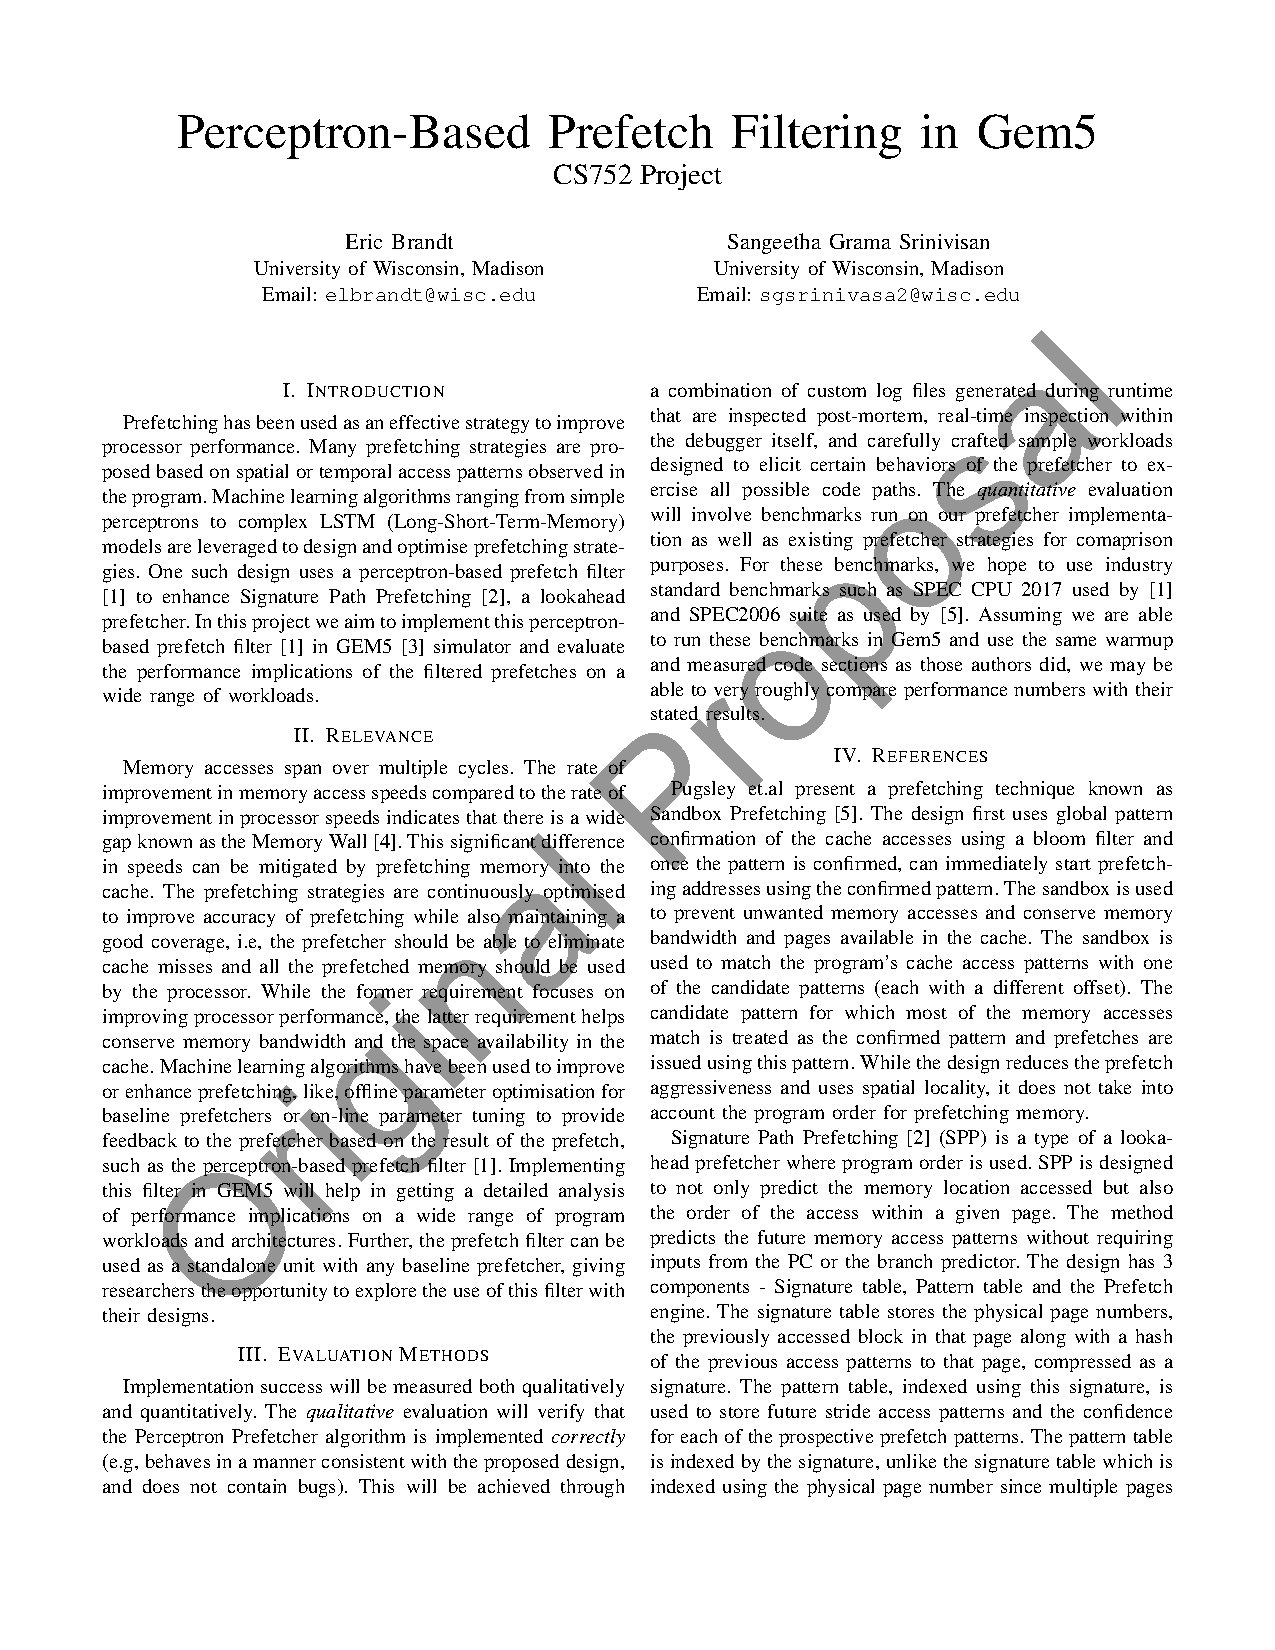
\includepdf[pages={1-3}]{BrandtSrinivisan_CS752ProjectProposal-watermarked.pdf}

% that's all folks
\end{document}

